\documentclass{standalone}

\usepackage[english]{babel} % English language/hyphenation
\usepackage{clock} % Required for generation clock icon
\ClockFrametrue\ClockStyle=3 % Format the clock icons
\usepackage{gensymb} % gives the degree symbol
\usepackage{graphicx} % Required for including pictures
\usepackage{tikz} % Required for drawing custom shapes
\usetikzlibrary{arrows}
\usetikzlibrary{shapes.misc}
\usetikzlibrary{decorations.pathreplacing}

\begin{document}
	\def\glider#1#2#3{
		\begin{scope}[shift={#1}, rotate=#2, scale=#3]
			\fill[black](0,0) -- (1,0) -- (1,1) -- (0,1) -- cycle;
			\fill[black](8/7+0,0) -- (8/7+1,0) -- (8/7+1,1) -- (8/7+0,1) -- cycle;
			\fill[black](16/7+0,0) -- (16/7+1,0) -- (16/7+1,1) -- (16/7+0,1) -- cycle;
			\fill[black](16/7+0,8/7+0) -- (16/7+1,8/7+0) -- (16/7+1,8/7+1) -- (16/7+0,8/7+1) -- cycle;
			\fill[black](8/7+0,16/7+0) -- (8/7+1,16/7+0) -- (8/7+1,16/7+1) -- (8/7+0,16/7+1) -- cycle;
		\end{scope}
	}
	\def\lwss#1#2#3{
		\begin{scope}[shift={#1}, rotate=#2, scale=#3]
			\fill[black](0,0) -- (1,0) -- (1,1) -- (0,1) -- cycle;
			\fill[black](8/7+0,0) -- (8/7+1,0) -- (8/7+1,1) -- (8/7+0,1) -- cycle;
			\fill[black](16/7+0,0) -- (16/7+1,0) -- (16/7+1,1) -- (16/7+0,1) -- cycle;
			\fill[black](24/7+0,0) -- (24/7+1,0) -- (24/7+1,1) -- (24/7+0,1) -- cycle;
			\fill[black](32/7+0,8/7+0) -- (32/7+1,8/7+0) -- (32/7+1,8/7+1) -- (32/7+0,8/7+1) -- cycle;
			\fill[black](0,8/7+0) -- (1,8/7+0) -- (1,8/7+1) -- (0,8/7+1) -- cycle;
			\fill[black](0,16/7+0) -- (1,16/7+0) -- (1,16/7+1) -- (0,16/7+1) -- cycle;
			\fill[black](8/7+0,24/7+0) -- (8/7+1,24/7+0) -- (8/7+1,24/7+1) -- (8/7+0,24/7+1) -- cycle;
			\fill[black](32/7+0,24/7+0) -- (32/7+1,24/7+0) -- (32/7+1,24/7+1) -- (32/7+0,24/7+1) -- cycle;
		\end{scope}
	}
	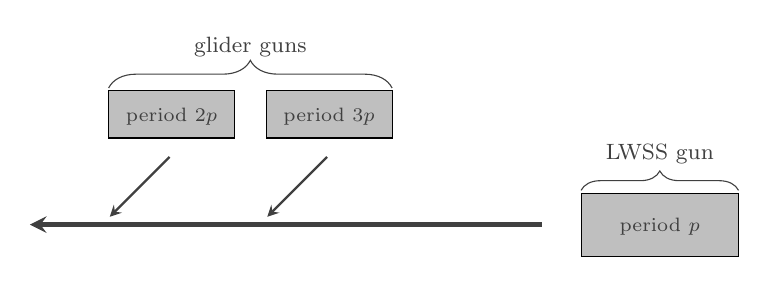
\begin{tikzpicture}%
		% GUNS
		\filldraw[color=black,fill=gray!50] (0,0) -- (1.6,0) -- (1.6,0.6) -- (0,0.6) -- cycle;
		\draw[darkgray] (0.8,0.27) node {\scriptsize period~$2p$};
		\filldraw[color=black,fill=gray!50] (2,0) -- (3.6,0) -- (3.6,0.6) -- (2,0.6) -- cycle;
		\draw[darkgray] (2.8,0.27) node {\scriptsize period~$3p$};
		
		\draw[darkgray,decorate,decoration={brace,amplitude=10pt},yshift=1pt]
		(0,0.6) --node [anchor=north,yshift=22pt]{\footnotesize glider guns} (3.6,0.6);
		
		% GLIDERS from GUNS
		\draw[thick,color=darkgray,-stealth] (0.775,-0.24) -- (0.015,-1);
		\glider{(0.7,-0.05)}{270}{0.08};
		\draw[thick,color=darkgray,-stealth] (2.775,-0.24) -- (2.015,-1);
		\glider{(2.7,-0.05)}{270}{0.08};
		
		% LWSS GUN
		\filldraw[color=black,fill=gray!50] (6,-0.7) -- (8,-0.7) -- (8,-1.5) -- (6,-1.5) -- cycle;
		\draw[darkgray] (7,-1.13) node {\scriptsize period~$p$};
		
		\draw[darkgray,decorate,decoration={brace,amplitude=7pt},yshift=1pt]
		(6,-0.7) --node [anchor=north,yshift=20pt]{\footnotesize LWSS gun} (8,-0.7);
		
		% LWSS from GUN
		\draw[ultra thick,color=darkgray,-stealth] (5.5,-1.1) -- (-1,-1.1);
		\lwss{(5.5,-1.23)}{0}{0.08};
	\end{tikzpicture}
\end{document}